\chapter{Конструкторский раздел}
\label{cha:design}

\section{Разработка алгоритма}
Рассмотренный алгоритм GSP в основном используется в торговли, и обычно под транзакцией имеется ввиду покупка определенного набора товаров (продуктов, книг и т.д.). В случае анализа активности пользователей САПР, зачастую, данные представлены в виде последовательности команд с параметрами, выполненных в определенный момент времени. Кроме этого, данный алгоритм учитывает кто совершил покупку, то есть id клиента.
Поэтому за одну транзакцию примем выполнение одной команды, а за id клиента - id сессии. В таком случае поддержкой последовательности команд будет отношение числа сессий поддерживающих данную последовательность к общему их количеству. 

Ключевые этапы:
Генерация кандидатов

\begin{figure}[h!]
	\centering
	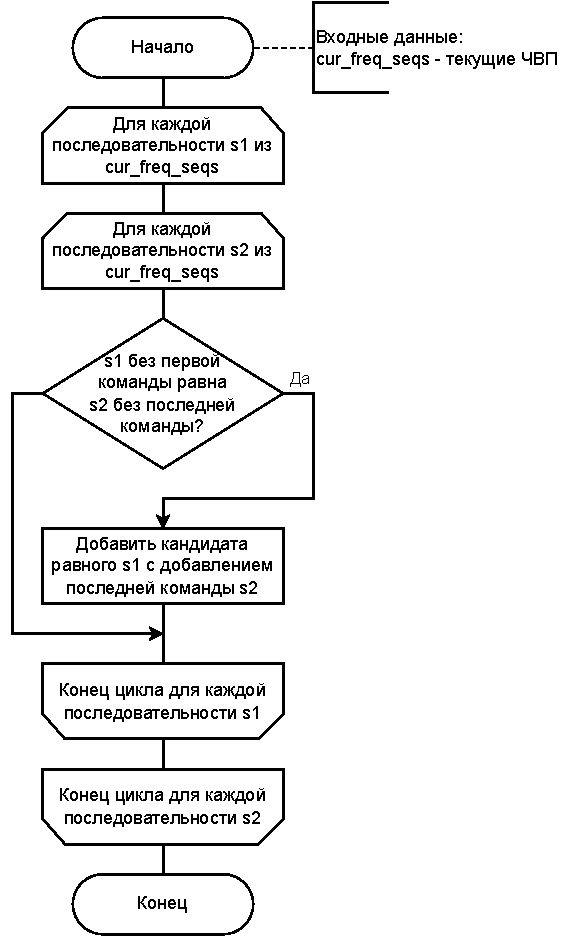
\includegraphics[width=0.7\textwidth]{inc/img/generateCandidates.drawio.pdf}
	\caption{Генерация кандидатов}
	\label{generateCandidates}
\end{figure}

Подсчет поддержки кандидатов

\begin{figure}[h!]
	\centering
	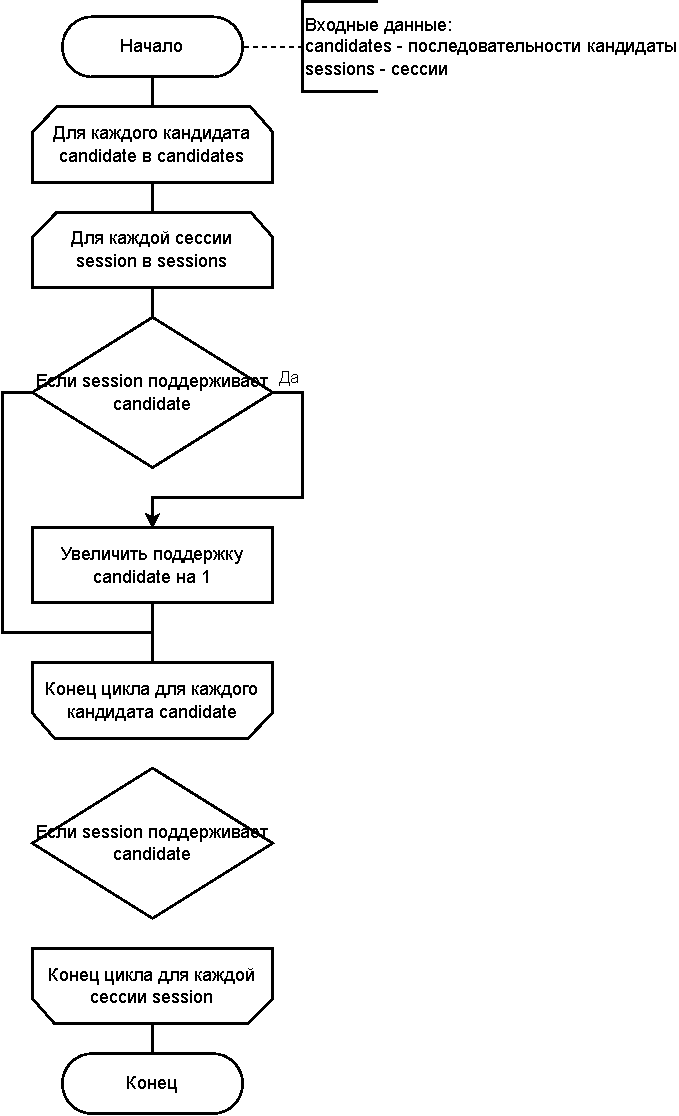
\includegraphics[width=0.8\textwidth]{inc/img/countSupport.drawio.pdf}
	\caption{Подсчет поддержки кандидатов}
	\label{countSupport}
\end{figure}

\begin{figure}[h!]
	\centering
	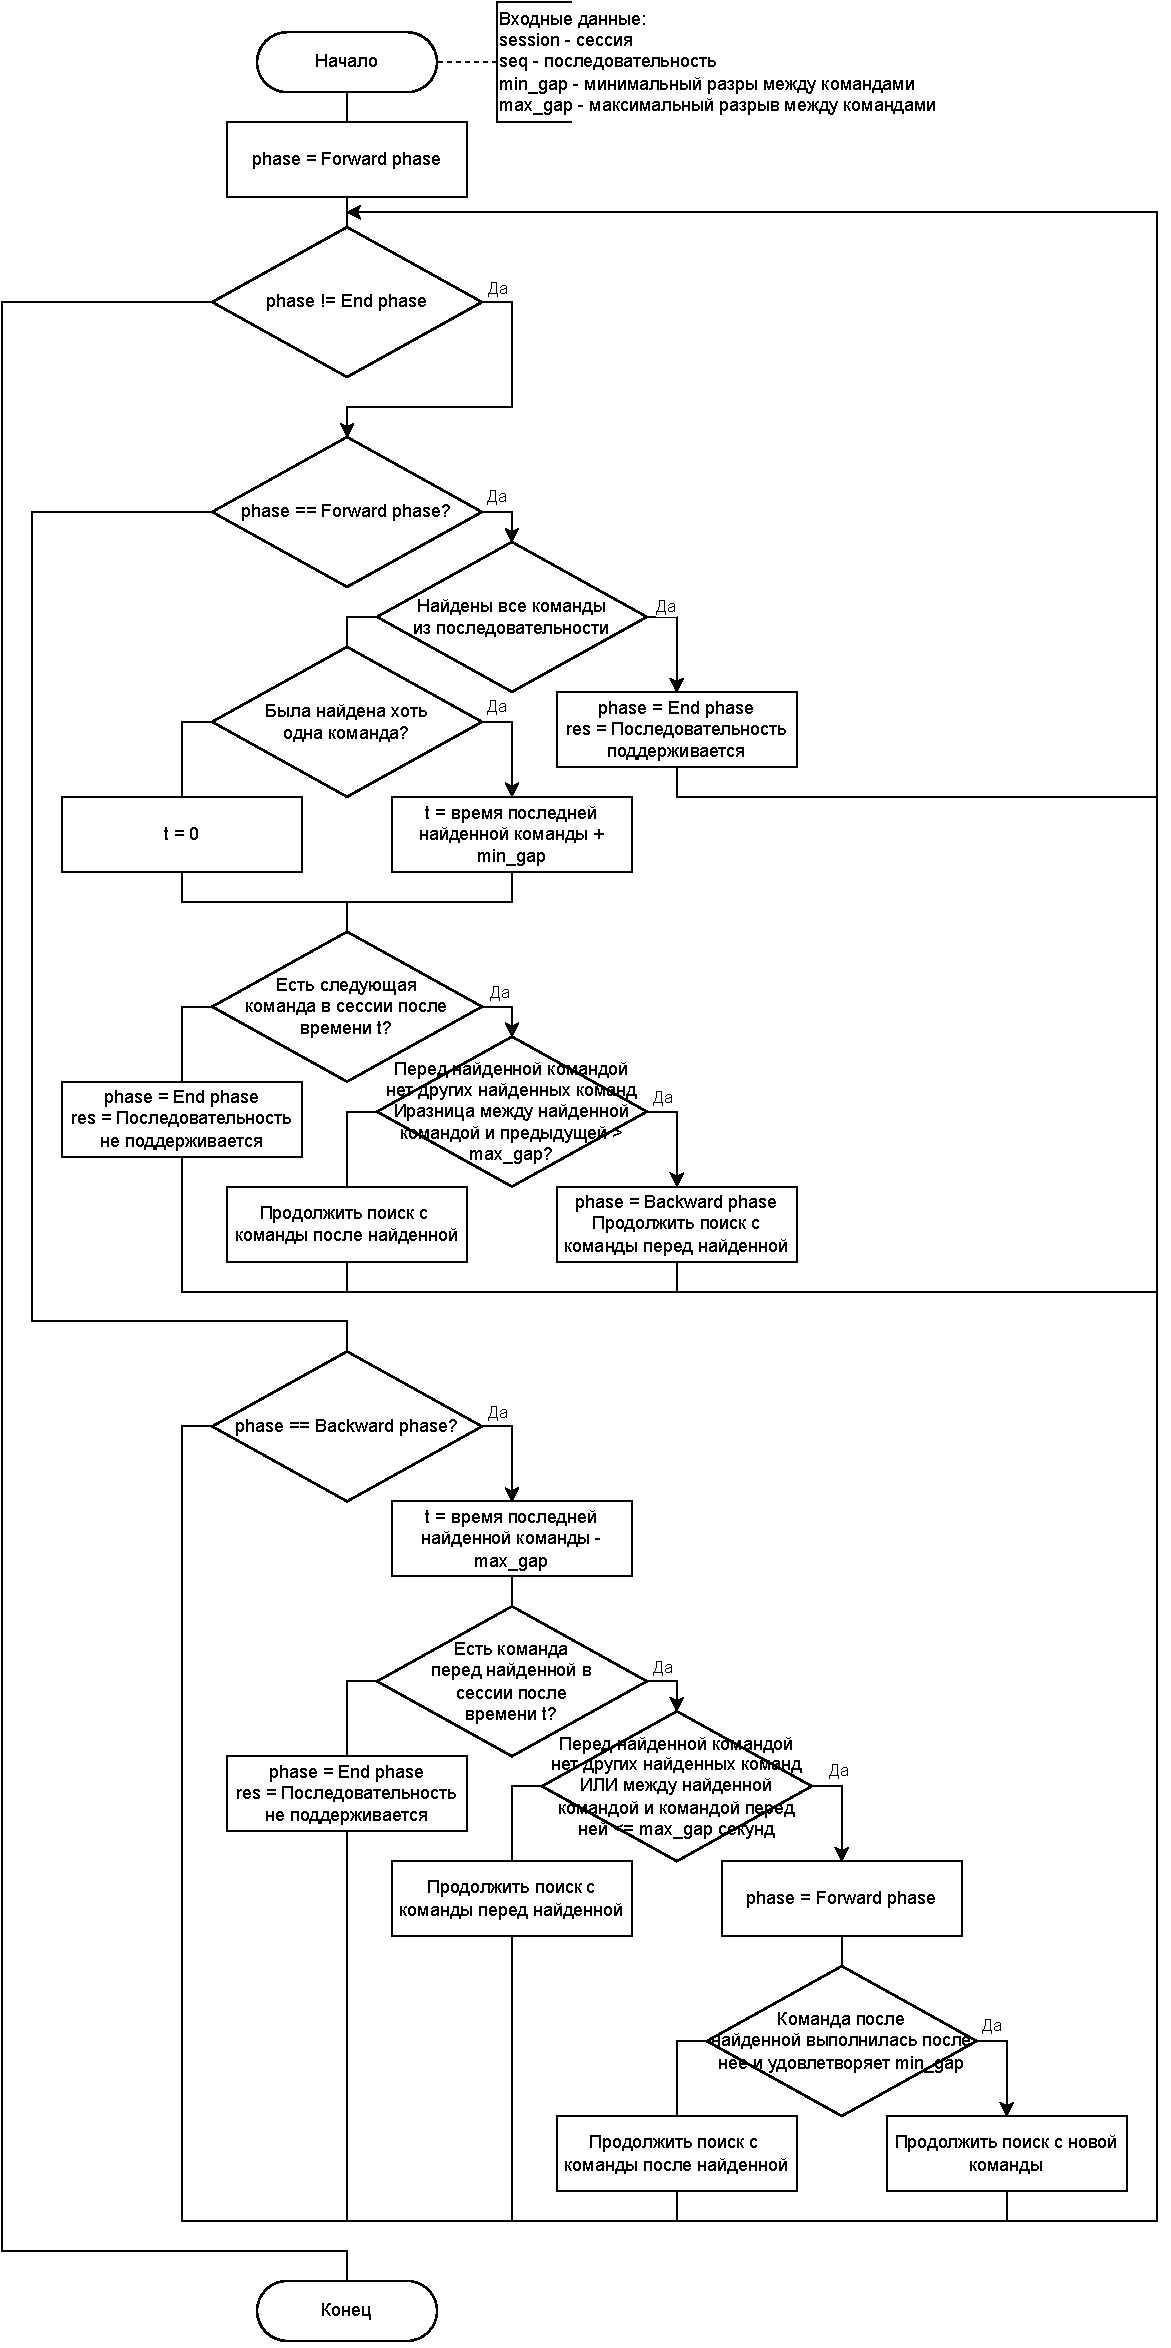
\includegraphics[width=0.7\textwidth]{inc/img/sessionSupportsSequence.drawio.pdf}
	\caption{Проверка поддержки кандидата сессией}
	\label{sessionSupportsSequence.drawio}
\end{figure}